% Metódy inžinierskej práce

\documentclass[10pt,slovak,a4paper]{article}

\usepackage[slovak]{babel}
%\usepackage[T1]{fontenc}
\usepackage[IL2]{fontenc} % lepšia sadzba písmena Ľ než v T1
\usepackage[utf8]{inputenc}
\usepackage{graphicx}
\usepackage{url} % príkaz \url na formátovanie URL
\usepackage{hyperref} % odkazy v texte budú aktívne (pri niektorých triedach dokumentov spôsobuje posun textu)

\usepackage{cite}
%\usepackage{times}

\pagestyle{plain}

\title{Sekvenčné UML Diagramy\thanks{Semestrálny projekt v predmete Metódy inžinierskej práce, ak. rok 2021/22, vedenie: Ing. Ján Lúčanský}}

\author{Kristián Lukacsovics\\[2pt]
    {\small Slovenská technická univerzita v Bratislave}\\
    {\small Fakulta informatiky a informačných technológií}\\
    {\small \texttt{xlukacsovics@stuba.sk}}
    }

\date{\small 14.12.2021}

\providecommand{\abstr}[1]{\textbf{\textit{Abstrakt---}} #1}
\providecommand{\keywords}[1]{\textbf{\textit{Klúčové slová---}} #1}

\begin{document}

\maketitle

\abstr{Tento článok sa zameriava na opis sekvenčných UML diagramov\ldots\newline}
\indent\keywords{Unified Modeling Language, Sekvenčný diagram, Objekt, Správa}

\section{Úvod}
\ldots

\section{Úroveň využitia}
UML, celým názvom Unified Modeling Language, je objektovo-orientovaný modelovací jazyk, ktorý slúži na modelovanie počítačových programov. \cite{eriksson98}
Existuje niekoľko typov UML diagramov, sekvenčné diagramy sú jedným z nich. Všetky tieto diagramy slúžia na
abstraktný opis správania sa jednotlivých častí počítačového programu. Každý jeden typ sa sústreďuje na opis
rôznych vlastností kódu. \cite{petraq14} \newline

\noindent Avšak, niektoré typy týchto diagramov sa využívajú v praxi viacej ako ostatné. Pri zistení popularity UML diagramov sa spravila zbierka niekoľko desiatok náučných
materiálov zamerané na UML. Medzi tieto materiály boli zaradené knihy, pomocné nástroje, kurzy a online tutoriály. Následne sa podľa počtu meteriálov, v ktorých boli spomenuté alebo použité
jednotlivé typy diagramov, percentuálne vyhodnotila úroveň využitia. Sekvenčné diagramy boli spomenuté alebo použité v 97 percentách materiálov, čím patrili medzi tie populárnejšie diagramy, spomedzi všetkých skúmaných diagramov. \cite{reggio13} \newline

\noindent Jednotlivé údaje z tejto štúdie môžeme vidieť na obr.~\ref{tab} .

\begin{figure*}[tbh]
\centering
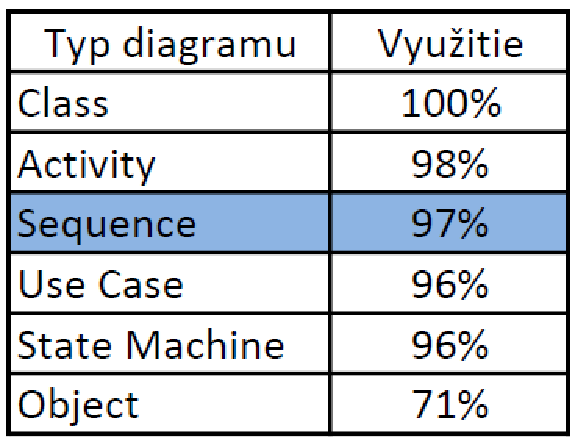
\includegraphics[scale=0.5]{tab.pdf}
\caption{Úroveň využitia jednotlivých typov UML diagramov. \cite{reggio13}}
\label{tab}
\end{figure*}

\section{Komunikácia objektov}

Ako už bolo spomenuté, UML diagramy sú objektovo-orientované, z čoho vyplýva, že základný prvok týchto diagramov je objekt. 
Medzi objektami nastávajú rôzne interakcie, ktorými vieme vyjadriť fungovanie programu, ktorý modelujeme. 
Pod interakciami môžeme rozumieť aj výmenu správ medzi objektami, pomocou ktorých medzi sebou komunikujú.
V prípade sekvenčných diagramov, sú tieto správy vyjadrené postupne ako sa udejú. Vďaka tomu je možné vyjadriť aj dĺžku života objektov. 
Ak daný objekt potrebuje, po prvýkrát, odoslať alebo obdržať správu, tento moment môžeme brať ako vytvorenie objektu. Podobným spôsobom vieme určiť aj moment odstránenia objektu.   
Treba dbať aj na poradie správ. Zmena poradia môže zmeniť korektnosť programu v niektorých prípadoch. \cite{petraq14} \newline

\noindent Správy sa v diagrame zaznačia ako horizontálne šípky. Smer týchto šípok určuje odosielateľa a
príjemcu správy (na strane, kde je šípka, je príjemca). Objekty si môžu poslať správy aj pre seba. Takéto správy sa nazývajú reflexívne správy. \cite{petraq14} 
Ak sa pošle správa s požiadavkou, návratová správa s odpoveďou od príjemcu požiadavky sa značí bodkovanou čiarou. 
Návratové správy majú otvorený hrot šípky narozdiel od ostatných správ, ktoré majú hrot zaplnený čiernou farbou. \cite{booch00}\newline

\noindent Samotné objekty sa značia ako obdĺžniky, do ktorých sa napíše meno objektu a meno inštancie objektu. Pod tieto obdĺžniky sa zaznačí vertikálna prerušovaná čiara. 
Úseky tejto čiary, kde je objekt aktívny (objekt bol vytvorený a nebol ešte odstránený) sa značí prázdnym obdĺžnikom. Správy sa kreslia zo stien týchto obdĺžnikov. \cite{booch00} \newline

\noindent Všetky tieto označenia pre objekty a správy sa ohraničia obdĺžnikom, ktorý slúži na oddelenie jednotlivých diagramov.
Do ľavého horného rohu tohto obdĺžnika sa píše meno diagramu. \cite{booch00}
Na obr.~\ref{diag1} je jednoduchá ukážka sekvenčného diagramu.

\begin{figure*}[tbh]
\centering
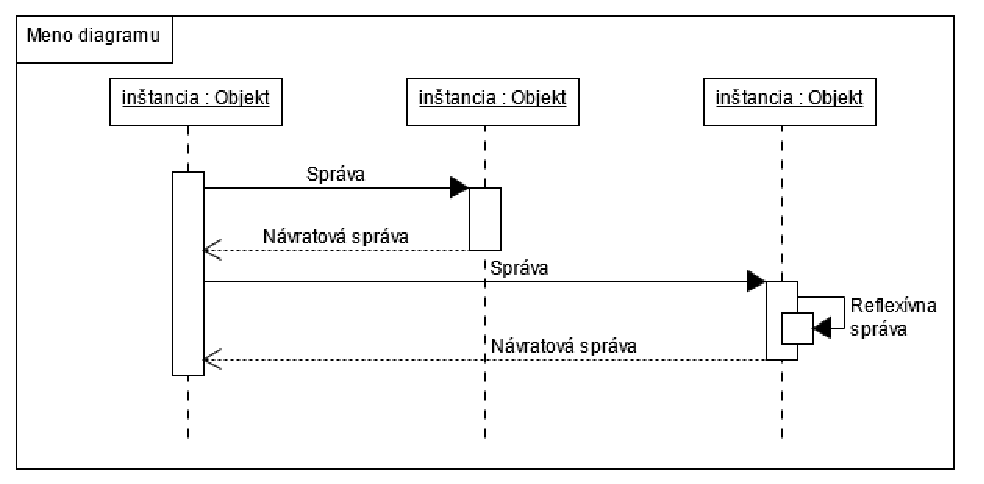
\includegraphics[scale=0.8]{simple_diag.pdf}
\caption{Ukážka sekvenčného diagramu.\cite{booch00}}
\label{diag1}
\end{figure*}

\section{Zložitejšie koncepty}

Pomocou sekvenčných diagramov vieme vyjadriť aj zložitejšie koncepty, ako sú napríklad cykly a podmienky. Na vyjadrenie týchto konceptov môžeme použiť tzv. kombinované fragmenty.
Kombinované fragmenty slúžia na zoskupenie správ podľa nejakého kritéria. 
Kombinované fragmenty sa v diagrame značia rovnako ako sa značia oddelenia diagramov. Správy sa ohraničia obdĺžnikom a do ľavého horného rohu obdĺžnika sa napíše meno 
kombinovaného fragmentu. Existuje niekoľko typov kombinovaných fragmentov, ako sú napr. cykly, voľby a alternatívy. \cite{booch00} \newline

\noindent Cykly zaznačujeme do diagramov ich anglickým názvom „loop". Pod meno sa do hranatých zátvoriek píše podmienka, ktorá sa overí na začiatku každej iterácie cyklu. 
Ak je podmienka splnená, spustí sa nová iterácia. 
Napr., ak by sme mali cyklus, v ktorom máme prejsť celý jeden spájaný zoznam, podmienka cyklu by bola zapísaná takto: „[node != NULL]". \cite{booch00} \newline

\noindent Pomocou volieb modelujeme vetvenie programu. Podmienka vetvenia sa značí rovnako ako podmienka pri cykloch. 
Označujú sa menom „opt" (skratka pre angl. slovo „options"). \cite{booch00} \newline

\noindent Alternatívy, takisto ako voľby, modelujú vetvenie programu, ale modelujú také vetvenie, v ktorom sa používa viac než jedna podmienka. 
Označujú sa menom „alt" (skratka pre angl. slovo „alternatives"). 
Príklad modelu alternatívy môžeme vidieť na obr.~\ref{diag2} . \cite{booch00} \newline

\noindent forsen

\begin{figure*}[tbh]
\centering
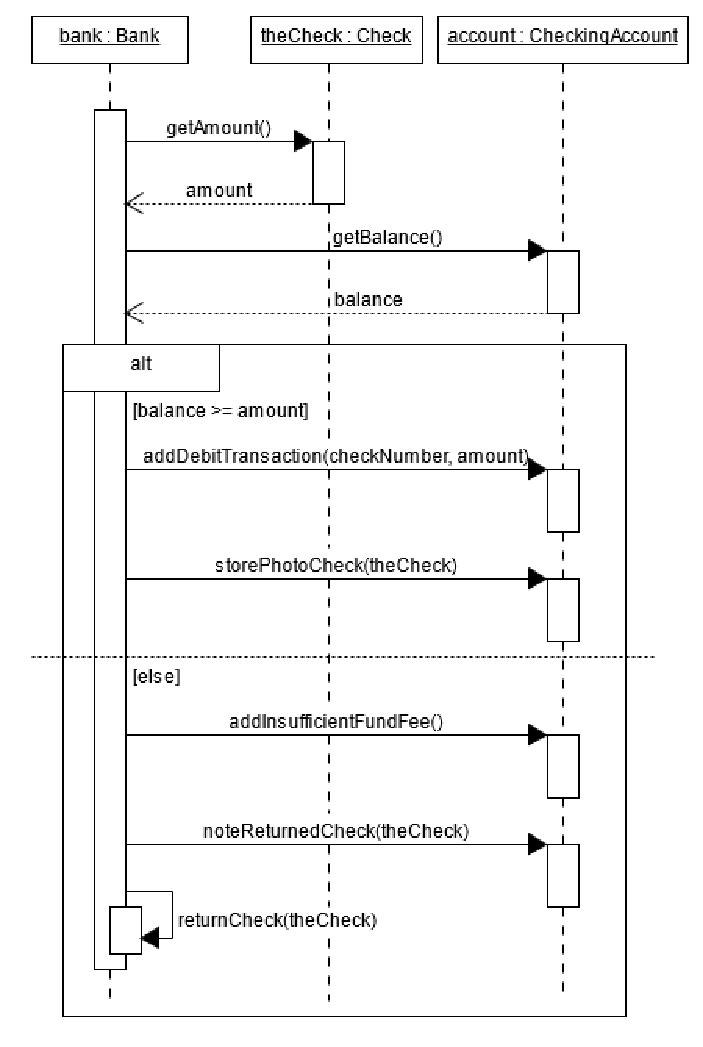
\includegraphics[scale=0.8]{cond_diag.pdf}
\caption{Model programu s alternatívou. \cite{booch00}}
\label{diag2}
\end{figure*}

\section{Reakcia na témy z prednášok}
\paragraph{Spoločenské súvislosti.}
\ldots

\paragraph{Historické súvislosti.}
\ldots

\paragraph{Technológia a ľudia.}
\ldots

\paragraph{Udržateľnosť a etika.}
\ldots

\section{Záver}
\ldots

% týmto sa generuje zoznam literatúry z obsahu súboru literature.bib podľa toho, na čo sa v článku odkazujete
\bibliography{literature}
\bibliographystyle{plain} % prípadne alpha, abbrv alebo hociktorý iný
\end{document}
